\documentclass[sigconf]{acmart}
\usepackage{booktabs}


%% \BibTeX command to typeset BibTeX logo in the docs
\AtBeginDocument{%
  \providecommand\BibTeX{{%
    \normalfont B\kern-0.5em{\scshape i\kern-0.25em b}\kern-0.8em\TeX}}}

%% These commands are for a PROCEEDINGS abstract or paper.
\settopmatter{printacmref=false} % Removes citation information below abstract
\renewcommand\footnotetextcopyrightpermission[1]{} % removes footnote with conference information in 

\acmConference[AEPRO 2022]{AEPRO 2022: Algorithm Engineering Projects}{March 1}{Jena, Germany}
% convert text to title case
% http://individed.com/code/to-title-case/

\begin{document}

%%
%% The "title" command has an optional parameter,
%% allowing the author to define a "short title" to be used in page headers.
\title[Simple Algorithms for Cleaning Scanned Document Images]{Simple Algorithms for Cleaning Scanned Document Images\\\large Algorithm Engineering 2022 Project Paper}

%%
%% The "author" command and its associated commands are used to define
%% the authors and their affiliations.

\author{Farin Lippmann}
\affiliation{%
  \institution{Friedrich Schiller University Jena}
  \country{Germany}}
\email{farin.lippmann@uni-jena.de}

%% The abstract is a short summary of the work to be presented in the article.
\begin{abstract}
Scanned or photographed document images often contain unwanted noise. This noise causes ink waste when printing and hinders both human readability and possible further processing steps. As a free, simple alternative to other tools for cleaning scanned document images, we present a set of simple but effective and efficient algorithms to clean document images by removing their noise, packaged in a command-line executable program. We found that applying multiple of these simple algorithms in sequence allowed us to adapt and reliably remove noise in many use cases.
\end{abstract}

%%
%% Keywords. The author(s) should pick words that accurately describe
%% the work being presented. Separate the keywords with commas.
\keywords{scanned document cleaning, noise removal, background removal}


%%
%% This command processes the author and affiliation and title
%% information and builds the first part of the formatted document.
\maketitle

\let\thefootnote\relax\footnotetext{AEPRO 2022, March 1, Jena, Germany. Copyright \copyright 2022 for this paper by its authors. Use permitted under Creative Commons License Attribution 4.0 International (CC BY 4.0).}


\section{Introduction}
As more and more document-related work is digitalized, many documents are scanned or photographed to process on computers. During this scanning or photographing, noise is introduced to the image. Noise is information that does not belong to the text. It can consist of an unwanted image background or high-frequency noise, which is generated during image capture. Noise causes ink waste when printing the documents and hinders both human readability and possible further processing steps like optical character recognition.

Since most tools to remove noise from scanned document images either cost money or are hard to use due to their complexity, we present a set of algorithms to remove noise from scanned document images. The task of noise removal will be split into two subtasks. Filters, the first category of algorithms, deal with removing high-frequency noise from an image, while the second category, thresholding techniques, are able to remove a document image's background, especially shadows, while keeping the text intact.


\subsection{Background}
Digital color images are typically encoded as large arrays of pixels, where each pixel's color is determined by three numbers, representing the red, green and blue part of the color respectively. Each of these values is represented as an integer in the interval $[0, 255]$. In this paper, the input image will be called $A$, with $A[i,j,c]$ denoting the $c$-th color value of the pixel in row $i$ and column $j$. $A[i,j]$ represents the tuple containing the pixel's color values. Also, $A[i-r...i+r, j-r...j+r]$ denotes the $(2r+1) \times (2r+1)$ subarray around the pixel in row $i$, column $j$. The output image will be called $B$ and indexed in the same way.

\subsection{Related Work}
This paper uses algorithms that are well established in image processing, like image filters and thresholding techniques. Image filters are commonplace in image processing applications and are found in standard textbooks on the subject, such as \cite{overview_book}. An overview of them can also be found in \cite{overview_paper}. The algorithm for the median filter is taken from the influential paper by Huang, \cite{huang}. The adaptive thresholding algorithm for background removal is also well established, further information can be found in \cite{thresholding}.

\subsection{Outline}
This paper is organized as follows. We start in section 2 by describing each of the algorithms along with their use cases and optimizations. In section 3 we review the strengths and weaknesses of each algorithm and showcase their performance in an example application. The paper then concludes with a summary and a prospect for future work.

\section{The Algorithms}
\subsection{Overview}
We separate the task of cleaning a document image into two subtasks: removing high-frequency noise and removing the image background. The removal of high-frequency noise is carried out by filtering algorithms while the background removal is done using thresholding.

\subsection{High-Frequency Noise Removal}
High-Frequency noise is a random variation in color values often introduced to an image by electronic noise during the scanning or photographing process. The most frequently occurring types are gaussian noise and salt-and-pepper noise.

Gaussian noise is caused by a number of technical factors during the image capture, which add up to cause a statistically normally distributed error in pixel color values.

Salt-and-pepper noise, also called impulse or spike noise, manifests as solitary pixels that are much brighter or darker than their surroundings. It can be caused, for example, by errors during analog-to-digital conversion, though it can also stem from dirt on the document or the image capturing device.

\subsubsection{Mean Filter}
Both types of high-frequency noise can be removed using filtering algorithms. The first of these is the mean filter. The mean filter is a convolutional filter that replaces each pixel with the mean of the pixels in a square with a given radius $r$ around it. This mean operation is carried out separately for each color channel.
$$
B[i,j,c] = \text{mean}(A[(i-r)..(i+r), (j-r)..(j+r), c])
$$
This calculation can be optimized by separating it into two phases: a horizontal and a vertical pass. In the horizontal pass, each element is replaced by the mean of the $2r+1$ elements surrounding it horizontally in the same row. The vertical pass then computes the mean of the vertical column surroundings. In the naive version, $(2r+1)^2$ values are added together for each pixel. In the optimized version, only $2 \cdot (2r+1)$ are needed.

The mean filter reliably removes gaussian noise but may produce some artifacts for large radii. This problem is solved by the gaussian filter.

\subsubsection{Gaussian Filter}
The gaussian filter is very similar to the mean filter. It also replaces each pixel with the mean of the pixels in a square around it, but it uses a gaussian-weighted mean. This way, pixels that are closer to the center are given more influence on the value, which makes the gaussian a true low-pass filter, unlike the mean. The naive way to compute the filter starts by creating a $(2r+1) \times (2r+1)$ array $W$ containing gaussian weights, centered on the middle element. To compute one pixel's new value, each of the pixels in the radius surrounding it is multiplied by it's corresponding element in $W$ before calculating the mean by summing up the values and dividing by the sum of the weights.
$$
B[i,j,c] = \text{mean}(W*A[(i-r)..(i+r), (j-r)..(j+r), c])
$$
Where $*$ is element-wise multiplication.

The calculation can be optimized in the same way the mean filter can, by splitting the operation into a vertical and a horizontal pass. The weights $W$ then become a one-dimensional array of $r$ gaussian weights.

Both the mean- and the gaussian filter are able to remove gaussian noise, with the mean filter trading the possibility of artifacts with large radii for some performance. Both filters however have the problem of blurring the image, especially for larger radii, and neither is able to reliably remove salt-and-pepper noise. Both of these problems are solved by the median filter.

\subsubsection{Median Filter}
The median filter follows a similar idea to the previous two filters. It replaces each pixel with the median value of it's surroundings. This allows it to remove salt-and-pepper noise and leaves the image's edges intact, blurring it much less than the mean or gaussian filter. Naively, the algorithm is implemented by sorting the surrounding elements of each pixel, using the sorted list to find the median.
$$
B[i,j,c] = \text{sort}(A[(i-r)..(i+r), (j-r)..(j+r), c])[\lfloor\frac{(2r+1)^2}{2}\rfloor]
$$
The algorithm can be optimized heavily by using a sliding histogram. A histogram is used to count the number of times each color value appears in a part of an image. For each row of the image, the histogram is initialized with a zero for each color value from 0 to 255. Then, going through the row column by column, pixels are added to the histogram when they enter the surrounding square and removed when they leave it as the surrounding square moves on. A visualization of this is seen in figure \ref{fig:medianfilter}. For each pixel, the median is computed using the histogram. Computing the median in a histogram is easy, and especially fast when the previous median and the pixel values that left the histogram are known. Depending on whether the new median is smaller or larger than the last one, one simply moves up or down the histogram, until one finds the value where half of all values in the histogram are smaller than it, which is the median. For more information, see \cite{huang}.

\begin{figure}
  \centering
  \includegraphics[width=\linewidth]{./graphics/Medianfilter.png}
  \caption{Visualization of the sliding window histogram median filter. As the window moves from one pixel to the next, the pixel values that leave the window are removed from the histogram while the ones that enter are added.}
  \label{fig:medianfilter}
\end{figure}

\subsection{Image Background Removal}
Scanned document images may contain a background, e.g. consisting of shadows or discolored paper. To remove this background we employ thresholding algorithms.

\subsubsection{Global Thresholding}
Global thresholding is a very simple technique to remove an image's background. It relies on the existence of a clear separation between the brightness levels of the background and foreground. Given a threshold $t$, it sets each pixel's color to $(255,255,255)$ (white) if the pixel's intensity is higher than $t$. A pixel's intensity is simply the mean of it's three color values.
$$
B[i,j] = 
\begin{cases} 
    (255,255,255) & \text{if} \; \text{mean}(A[i,j]) > t \\
    A[i,j] &\text{otherwise}
\end{cases}
$$
The algorithm's simplicity gives it a good performance. However, it does not work if there is not a clear brightness separation between foreground and background, e.g. if there is a brightness gradient in the image. It also relies on the user to pick a fitting threshold $t$. Given a good threshold however, it may even work for document images that contain pictures, something that the following algorithm cannot.

\subsubsection{Adaptive Thresholding}
The reason why global thresholding cannot handle brightness gradients is that the same threshold is used for the whole image. Adaptive thresholding remedies this problem by computing a threshold $t$ for each pixel by taking the mean of the pixel's surroundings. For a cleaner separation, a given threshold gap $C$ is subtracted from the computed threshold. This way, a pixel needs to be significantly darker than it's surroundings to count as foreground. The mean may also be replaced by the gaussian weighted mean; this may lead to better results for some images.

\begin{align*}
    t &= \text{mean}(A[(i-r..i+r, j-r..j+r]) \\
    B[i,j] &= 
    \begin{cases} 
        (255,255,255) & \text{if} \; \text{mean}(A[i,j]) > t-C \\
        A[i,j] &\text{otherwise}
    \end{cases}
\end{align*}

A simple optimization for this algorithm is to compute all the means beforehand. In particular, the optimized mean filter and gaussian filter algorithms can be used for this purpose. Afterwards, only one more pass through the image is needed to compare pixel intensities with the means, taking roughly the same effort as global thresholding.

\section{Experiments}
The different algorithms have different strengths and weaknesses. Together they are able to clean most scanned document images, although some problems still need to be addressed. Figures 2 to 4 showcase the algorithms, all figures contain parts of the same example image, seen in full in figure \ref{fig:threshold}.

\begin{figure}
  \centering
  \includegraphics[width=\linewidth]{./graphics/filter_comparison_1.png}
  \caption{Example comparison between the different filtering algorithms on a document image with gaussian noise. Left: Original image, Middle Left: Mean filter with radius 1, Middle Right: Gaussian filter with radius 3, Right: Median filter with radius 1. Different radii were chosen to get approximately equal effects.}
  \label{fig:filtercomparison1}
\end{figure}

\begin{figure}
  \centering
  \includegraphics[width=\linewidth]{./graphics/filter_comparison_2.png}
  \caption{Example comparison between the mean and gaussian filter for large radii, showcasing the artifacts that the mean filter creates. Also visible are the dark borders that exist due to the naive edge case handling. Left: Mean filter with radius 4, Right: Gaussian filter with radius 9.}
  \label{fig:filtercomparison2}
\end{figure}

The mean filter is a simple and fast filter for removing gaussian noise, although it blurs the image and may create artifacts for large radii. The gaussian filter is slightly slower than the mean, but because it is a true low-pass filter, it does not create any artifacts, as is visible in figure \ref{fig:filtercomparison2}. Both the mean and the gaussian filter do not reliably remove salt-and-pepper noise and create dark edges at the borders of the image due to their naive edge case handling. The median filter is able to reliably remove salt-and-pepper noise and blurs the image less than the other filters, though it is a bit slower than them.

Adaptive thresholding is able to remove the background of text-only document images, even when there is a brightness gradient, but it will also remove parts of pictures in document images that contain them. It may also leave some dark speckles where the background had particularly dark pixels. Global thresholding is an alternative to use only when foreground and background have a clear brightness separation, as seen in figure \ref{fig:threshold}.

\begin{figure}
  \centering
  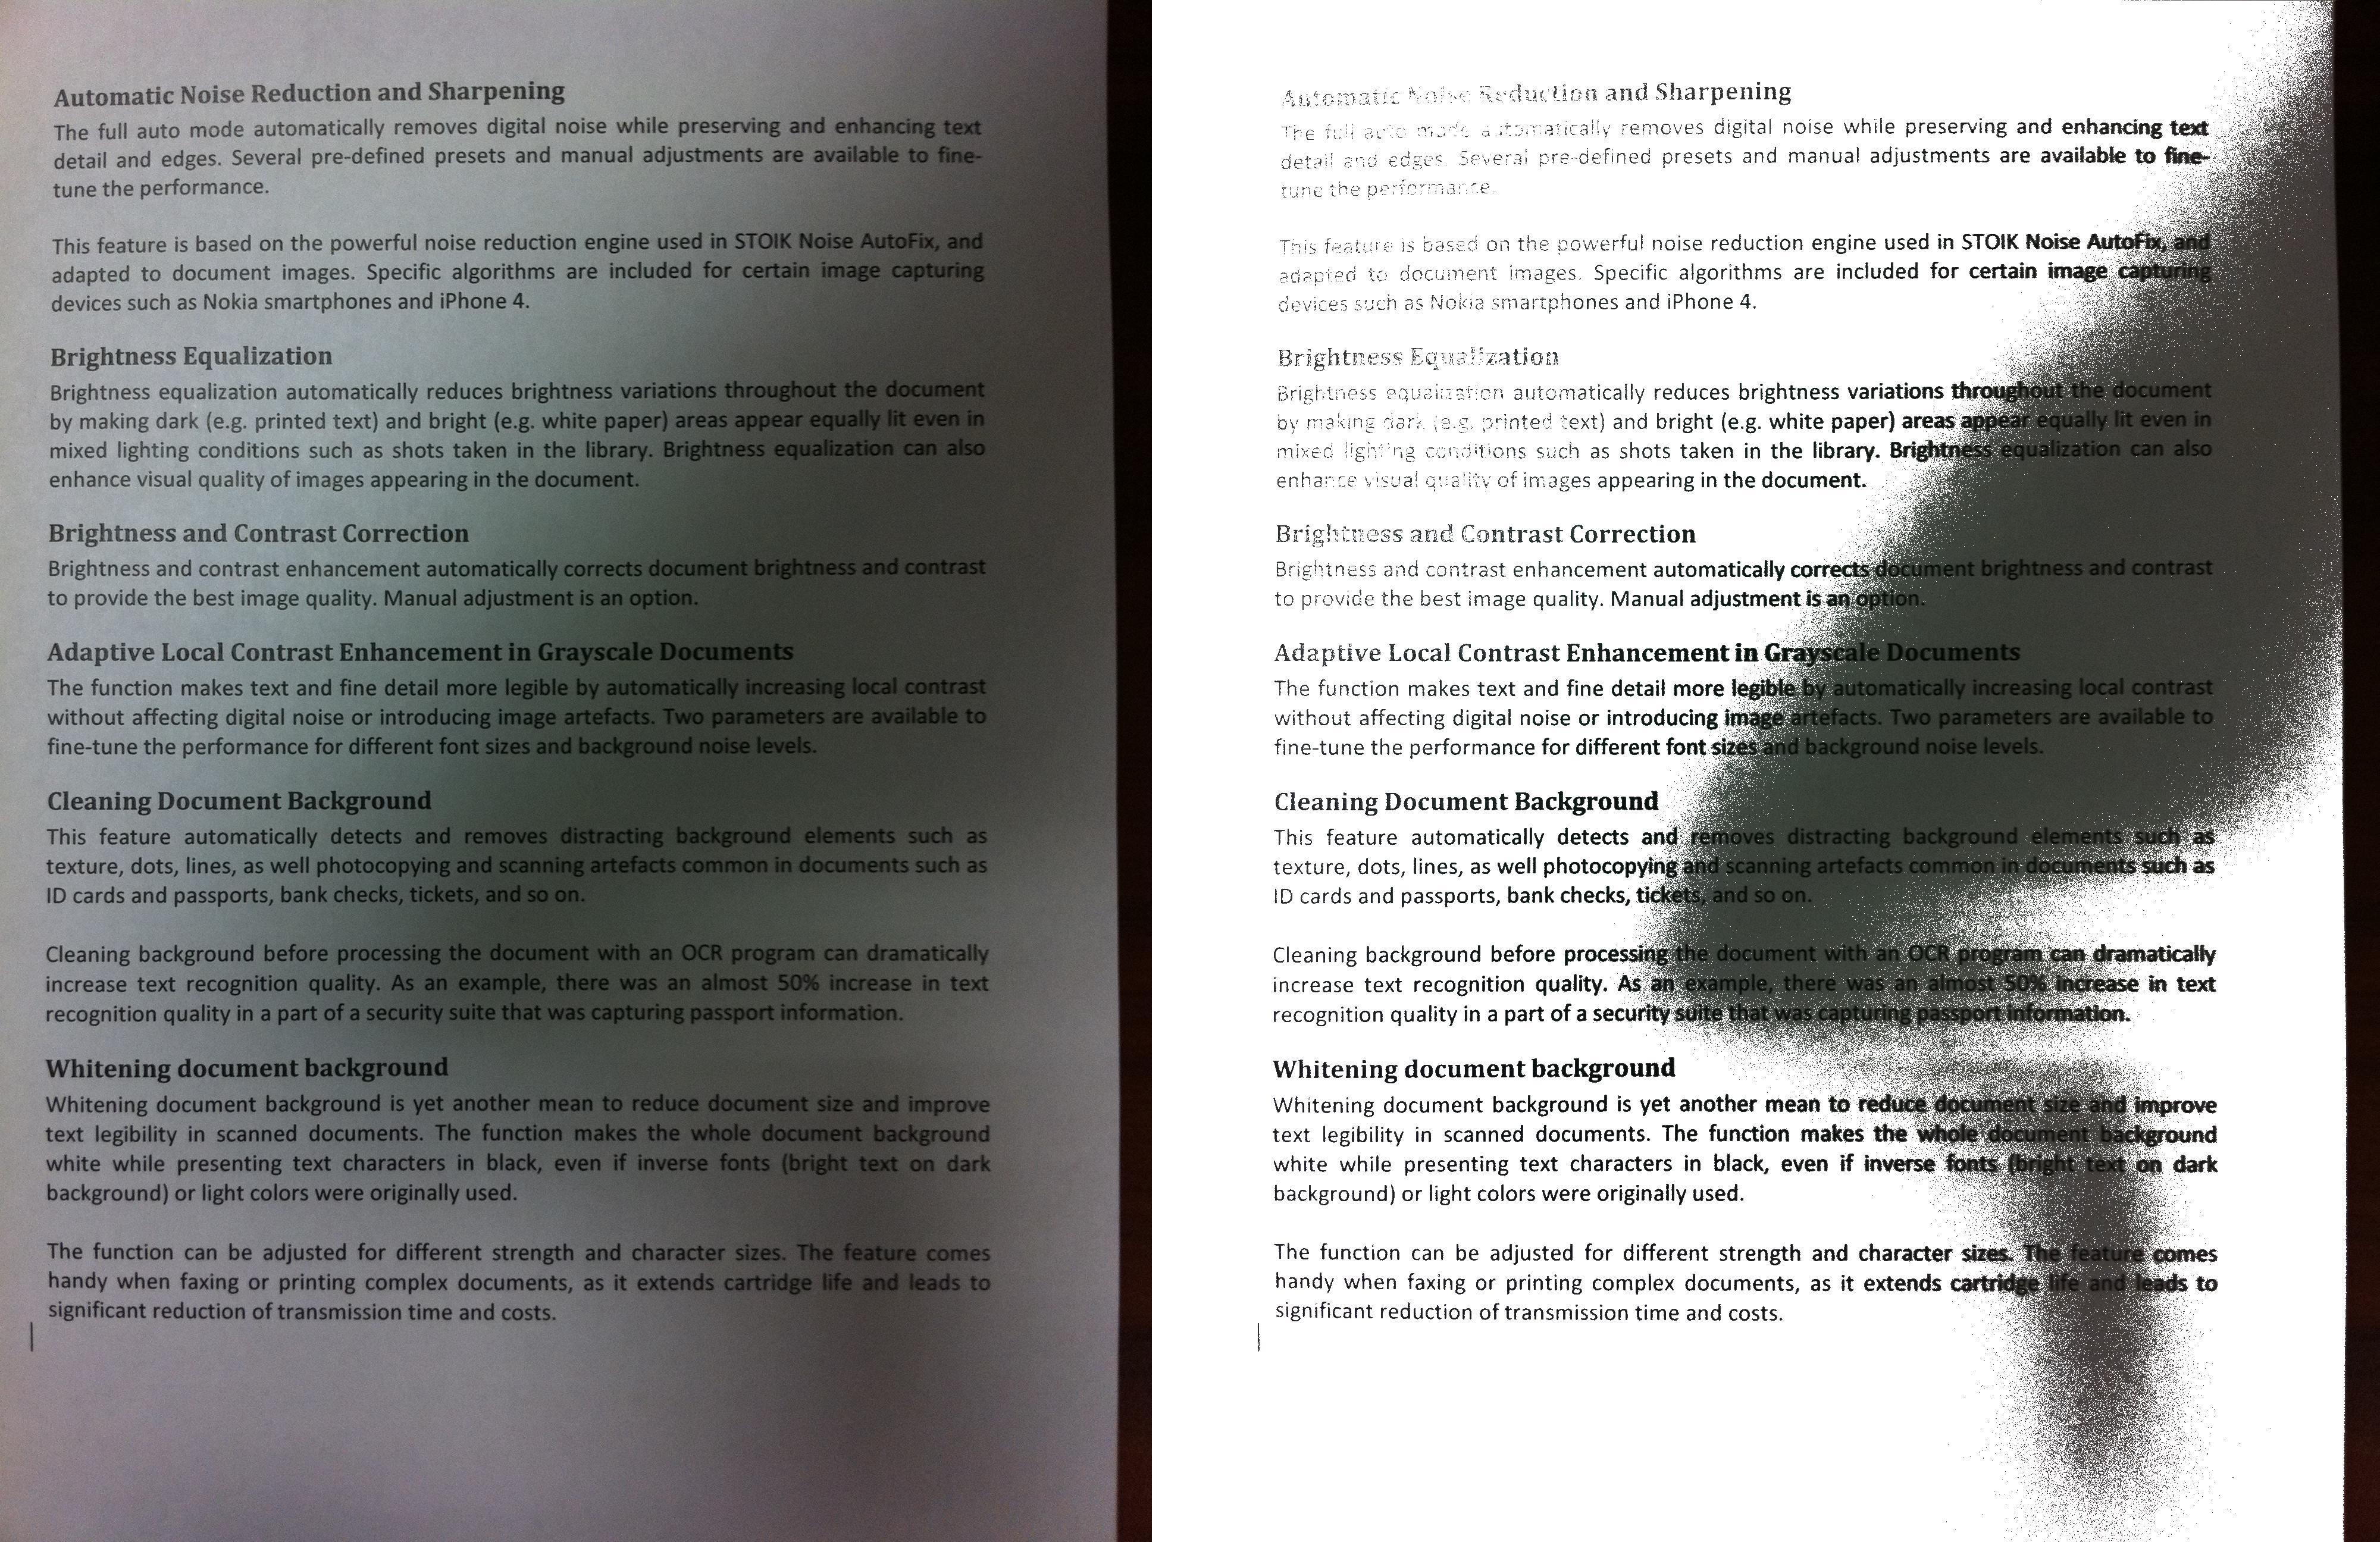
\includegraphics[width=\linewidth]{./graphics/threshold.png}
  \caption{Showcase of how global thresholding fails when a brightness gradient prevents a clear separation of fore- and background. Left: Original Image, Right: Global thresholding with threshold 70.}
  \label{fig:threshold}
\end{figure}

\begin{figure}
  \centering
  \includegraphics[width=\linewidth]{./graphics/threshold2.png}
  \caption{Showcase of adaptive mean and gaussian thresholding on the example image. Both versions remove the shadows even with a brightness gradient. The mean version leaves some speckles while the gaussian version slightly brightens the text where the shadow was. The original image is seen in figure \ref{fig:threshold}. Left: Adaptive mean threshold with radius 5 and C 10, Right: Adaptive gaussian threshold with radius 10 and C 2.}
  \label{fig:threshold2}
\end{figure}

After optimization, which includes parallelization, all algorithms run in reasonable time with commonly used parameters, as seen in table 1.  Cache optimization could not be employed due to the array-of-structs structure of color image data. As the image is saved as an array of pixels with each pixel containing three color values, accessing one color value from many pixels, which is the main type of access these algorithms use, is not possible in unit-stride. If better performance is required, an alternative image format may help in this regard.

\begin{table}[]
    \centering
    \begin{tabular}{c | c c}
        Parameters & Naive & Optimized \vspace{0.05cm} \\ \hline
        \multicolumn{3}{c}{\textbf{Mean Filter}} \\ \hline
        radius=1 & 0.705 & 0.300 \\
        radius=3 & 3.151 & 0.472 \\
        radius=5 & 7.682 & 0.682 \\ \hline
        \multicolumn{3}{c}{\textbf{Gaussian Filter}} \\  \hline
        radius=1 & 0.858 & 0.314 \\
        radius=3 & 4.187 & 0.557 \\
        radius=5 & 10.035 & 0.865 \\ \hline
        \multicolumn{3}{c}{\textbf{Median Filter}} \\  \hline
        radius=1 & 3.258 & 0.373 \\
        radius=3 & 38.017 & 0.770 \\
        radius=5 & 174.162 & 1.170 \\ \hline
        \multicolumn{3}{c}{\textbf{Global Threshold}} \\  \hline
        threshold=100 & 0.068 & 0.022 \\ \hline
        \multicolumn{3}{c}{\textbf{Adaptive Threshold Mean}} \\  \hline
        radius=2, C=10 & 1.611 & 0.401 \\
        radius=5, C=10 & 7.541 & 0.700 \\
        radius=10, C=10 & 27.846 & 1.182 \\ \hline
        \multicolumn{3}{c}{\textbf{Adaptive Threshold Gaussian}} \\  \hline
        radius=2, C=10 & 2.552 & 0.472 \\
        radius=5, C=10 & 11.534 & 0.877 \\
        radius=10, C=10 & 43.362 & 1.392 \\ \hline
    \end{tabular}
    \caption{Run times in seconds on the example image of size 1936 $\times$ 2592 using common parameter values. Measures were taken on a PC running Ubuntu 20.04 using an Intel Core i5 4460 CPU and 8GB of RAM.}
\end{table}

Best results could be seen when running multiple algorithms in sequence. For example, one might slightly smooth out an image using a mean or gaussian filter, which reduces the speckles that the following adaptive thresholding leaves. The few speckles that are created can be removed using a median filter. To finish, one might apply a gaussian filter to remove some of the letters' sharp and jagged edges that thresholding creates.


\section{Conclusions}
In this paper we showcased a set of algorithms for cleaning document images by removing their background and high-frequency noise. By applying multiple simple and efficient algorithms with different use cases in sequence, many types of document images can be cleaned.

Further improvements can be made in multiple places. For one, the image border cases are not handled well by the mean and gaussian filter, which could be fixed by interpolating the missing pixel values. Furthermore, we are currently missing an algorithm to use for background removal when the document contains an image and there is no clear brightness separation between fore- and background. To finish, another unsatisfied use case is the automatic correction of image orientation, useful when a document was placed askew under the scanner or photographed from an angle.

%%
%% The next two lines define the bibliography style to be used, and
%% the bibliography file.
\bibliographystyle{ACM-Reference-Format}
\bibliography{literature}


\end{document}
\endinput
%%
%% End of file `sample-sigconf.tex'.
